%!TEX TS-program = xelatex
%!TEX encoding = UTF-8 Unicode

\documentclass{beamer}
\usepackage{fontspec}
\usepackage{fontspec}
\usepackage{xunicode}
\usepackage{xltxtra}
\usepackage{xecyr}
\usepackage{hyperref}
\setmainfont[Mapping=tex-text]{DejaVu Serif}
\setsansfont[Mapping=tex-text]{DejaVu Sans}
\setmonofont[Mapping=tex-text]{DejaVu Sans Mono}
\usepackage{polyglossia}
\setdefaultlanguage{russian}
\usepackage{graphicx}
\usepackage{listings}

\mode<presentation> {
\usetheme{Warsaw}
\usecolortheme{dove}

\setbeamertemplate{footline}[page number]
%\setbeamertemplate{caption}[numbered]
\setbeamertemplate{caption}{\insertcaption}
}

\usepackage{graphicx} % Allows including images
\usepackage{booktabs} % Allows the use of \toprule, \midrule and \bottomrule in tables

%----------------------------------------------------------------------------------------
%	TITLE PAGE
%----------------------------------------------------------------------------------------
% The short title appears at the bottom of every slide, the full title is only on the title page
\title[Упражнения в Stepic]{Разработка системы проверки упражнений для
  образовательной платформы}
\author{Алексей Кладов\\
  { \footnotesize \textcolor{gray}{группа 545\\ руководитель Вяххи Н. И.}}}
\institute[СПбГУ]{Санкт-Петербургский государственный университет}
\date{\today} % Date, can be changed to a custom date

\begin{document}

\begin{frame}
\titlepage % Print the title page as the first slide
\end{frame}

%----------------------------------------------------------------------------------------
%	PRESENTATION SLIDES
%----------------------------------------------------------------------------------------
\begin{frame}{Stepic}
  \begin{columns}[t]
    \column{.5\textwidth}
    Статус
    \begin{itemize}
    \item 2013 год
    \item 23000 студентов
    \item 2 курса на Coursera
    \item курсы CS Center
    \end{itemize}

    \column{.5\textwidth}
    Технологии
    \begin{itemize}
    \item Linux
    \item Python 3, Django, Celery, Codejail
    \item Django \textbf{REST} framework
    \item CoffeeScript, Ember
    \end{itemize}
  \end{columns}

  \medskip

  Много студентов $\Rightarrow$
  \begin{itemize}
  \item Масштабирование лекций.
  \item Масштабирование \underline{упражнений}.
  \end{itemize}
\end{frame}

\begin{frame}{Постановка задачи}
  Реализовать \underline{расширяемую} систему для создания и проверки упражнений
  для образовательной платформы Stepic.

  \medskip

  Подзадачи
  \begin{itemize}
  \item Разработать фреймворк для расширения набора типов упражнений
    сторонними разработчиками.
  \item Реализовать с помощью фреймворка часто встречающиеся типы упражнений.
  \item Обеспечить масштабируемое и изолированное исполнение
    потенциально небезопасного кода упражнений.
  \end{itemize}
\end{frame}

\begin{frame}{Фреймворк}
  \begin{figure}
    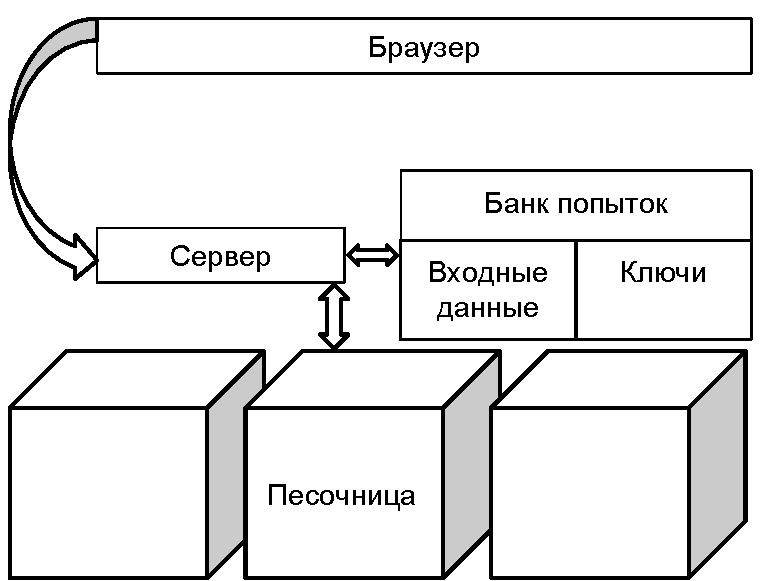
\includegraphics[width=0.8\textwidth]{../res/arch.pdf}
    \caption{Архитектура решения}
  \end{figure}

\end{frame}

\begin{frame}{Примеры типов упражнений}
  \begin{columns}
    \column{.5\textwidth}
    \begin{itemize}
    \item Choice
    \item \underline{Code}
    \item \underline{Dataset}
    \item Free Answer
    \item \underline{Math}
    \item Number
    \item Sorting
    \item \underline{String}
    \item \textbf{Admin}
    \end{itemize}
    Используются в текущих курсах!
    \column{.5\textwidth}
    \begin{figure}
      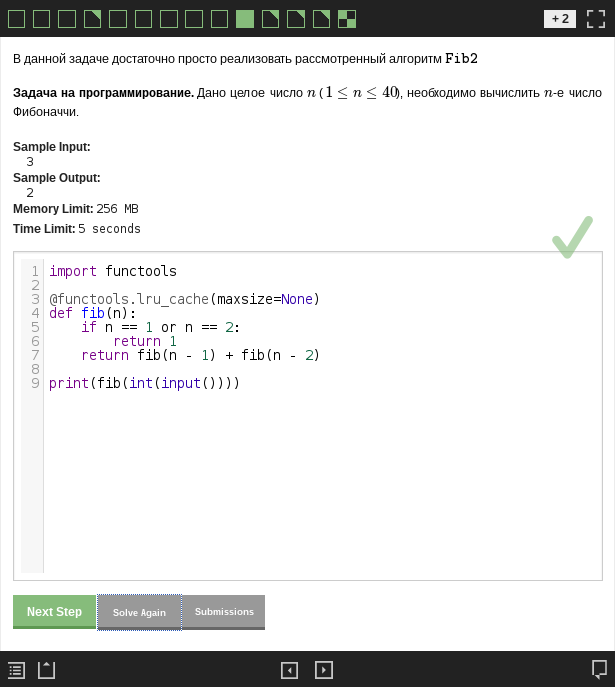
\includegraphics[width=\textwidth]{../res/quiz.png}
      \caption{Пример упражнения (Code)}
    \end{figure}
  \end{columns}
\end{frame}

\begin{frame}{Изоляция и масштабирование}
  \begin{itemize}
  \item Расширение Codejail (мультиязычность, сообщения об ошибках,
    коммуникация...)
  \item Создание профилей Apparmor.
  \item Масштабируемость при помощи Celery.
  \item Планы: управление конфигурациями.
  \end{itemize}
\end{frame}

\begin{frame}{Результаты}
  \begin{itemize}
  \item[\checkmark] Разработан фреймворк для создания новых типов упражнений.
  \item[\checkmark] С помощью фреймворка реализовано 9 типов упражнений, которые успешно использованы
    в крупных курсах. Один тип упражнения был разработан сторонним разработчиком.
  \item[\checkmark] На основе Celery и Codejail создана система масштабируемого и
    безопасного исполнения кода.
  \end{itemize}
\end{frame}

\end{document}

%%% Local Variables:
%%% coding: utf-8
%%% mode: latex
%%% TeX-engine: xetex
%%% End: